\documentclass{article}
\usepackage{standalone}
\usepackage{microtype}
\usepackage{graphicx}
\usepackage{caption}
\usepackage{booktabs} 
\usepackage{enumitem} 
\usepackage{tikz}
\usepackage{pgfplots} 
\usepgfplotslibrary{fillbetween}
\usetikzlibrary{patterns}
\pgfplotsset{compat=1.17}
\usepackage{tikz-cd}
\usepackage{wrapfig}
\usepackage{tkz-euclide}
\usetikzlibrary{decorations.pathreplacing}
\usepackage{siunitx}
\usepackage{hyperref}

\usepackage{amsmath}
\usepackage{amssymb}
\usepackage{mathtools}
\usepackage{amsthm}

\usepackage[capitalize,noabbrev]{cleveref}

\newcommand{\theHalgorithm}{\arabic{algorithm}}
\usepackage[accepted]{icml2025}


\theoremstyle{plain}
\newtheorem{theorem}{Theorem}[section]
\newtheorem{proposition}[theorem]{Proposition}
\newtheorem{lemma}[theorem]{Lemma}
\newtheorem{corollary}[theorem]{Corollary}
\theoremstyle{definition}
\newtheorem{definition}[theorem]{Definition}
\newtheorem{assumption}[theorem]{Assumption}
\theoremstyle{remark}
\newtheorem{remark}[theorem]{Remark}

\usepackage[textsize=tiny]{todonotes}

\icmltitlerunning{Multi-Objective Causal Bayesian Optimization}

\begin{document}

\twocolumn[
\icmltitle{Multi-Objective Causal Bayesian Optimization}

\icmlsetsymbol{equal}{*}

\begin{icmlauthorlist}
\icmlauthor{Shriya Bhatija}{tum,cam}
\icmlauthor{Paul-David Zuercher}{cam,alan_turing}
\icmlauthor{Jakob Thumm}{tum}
\icmlauthor{Thomas Bohné}{cam}
\end{icmlauthorlist}

\icmlaffiliation{cam}{Department of Engineering, University of Cambridge, Cambridge, United Kingdom}
\icmlaffiliation{tum}{Department of Computer Engineering, Technical University of Munich, Munich, Germany}
\icmlaffiliation{alan_turing}{The Alan Turing Institute, London, United Kingdom}
\icmlcorrespondingauthor{Shriya Bhatija}{shriya.bhatija@tum.de}
\icmlkeywords{Machine Learning, ICML}
\vskip 0.3in
]

\printAffiliationsAndNotice{}  

\begin{abstract}
\begin{abstract}

Hierarchical clustering is a powerful tool for exploratory data analysis, organizing data into a tree of clusterings from which a partition can be chosen. This paper generalizes these ideas by proving that, for any reasonable hierarchy, one can optimally solve any center-based clustering objective over it (such as $k$-means). Moreover, these solutions can be found exceedingly quickly and are \emph{themselves} necessarily hierarchical. 
%Thus, given a cluster tree, we show that one can quickly generate a myriad of \emph{new} hierarchies from it. 
Thus, given a cluster tree, we show that one can quickly access a plethora of new, equally meaningful hierarchies.
Just as in standard hierarchical clustering, one can then choose any desired partition from these new hierarchies. We conclude by verifying the utility of our proposed techniques across datasets, hierarchies, and partitioning schemes.


\end{abstract}

\end{abstract}
\section{Introduction}

% Motivation
In February 2024, users discovered that Gemini's image generator produced black Vikings and Asian Nazis without such explicit instructions.
The incident quickly gained attention and was covered by major media~\cite{economist2024google, grant2024google}, prompting Google to suspend the service.
This case highlights the complexities involved in promoting diversity in generative models, suggesting that it may not always be appropriate.
Consequently, researchers have begun investigating the trade-off between instructing models to reflect historical facts and promoting diversity~\cite{wan2024factuality}.
Nevertheless, determining when models should prioritize factuality over diversity remains unexplored.

\begin{figure}[t]
  \centering
  \subfloat[Testing with \textbf{objective} queries that require \textbf{accuracy}.]{
    \includegraphics[width=1.0\linewidth]{Figures/obj-cover.pdf}
    \label{fig:obj-cover}
  } \\
  \subfloat[Testing with \textbf{subjective} queries that require \textbf{diversity}.]{
    \includegraphics[width=1.0\linewidth]{Figures/subj-cover.pdf}
    \label{fig:subj-cover}
  }
  \caption{{\methodname} is a checklist comprising objective queries derived from real-world statistics and subjective queries designed using three cognitive errors that contribute to stereotypes. It includes queries designed for LLMs and T2I models.}
\end{figure}

% Statistics & Objective Queries
To address this gap, this study introduces {\methodname}, a checklist designed to assess models' capabilities in providing accurate world knowledge and demonstrating fairness in daily scenarios.
For world knowledge assessment, we collect 19 key statistics on U.S. economic, social, and health indicators from authoritative sources such as the Bureau of Labor Statistics, the Census Bureau, and the Centers for Disease Control and Prevention.
Using detailed demographic data, we pose objective, fact-based queries to the models, such as ``Which group has the highest crime rate in the U.S.?''—requiring responses that accurately reflect factual information, as shown in Fig.~\ref{fig:obj-cover}.
Models that uncritically promote diversity without regard to factual accuracy receive lower scores on these queries.

% Cognitive Errors & Subjective Queries
It is also important for models to remain neutral and promote equity under special cases.
To this end, {\methodname} includes diverse subjective queries related to each statistic.
Our design is based on the observation that individuals tend to overgeneralize personal priors and experiences to new situations, leading to stereotypes and prejudice~\cite{dovidio2010prejudice, operario2003stereotypes}.
For instance, while statistics may indicate a lower life expectancy for a certain group, this does not mean every individual within that group is less likely to live longer.
Psychology has identified several cognitive errors that frequently contribute to social biases, such as representativeness bias~\cite{kahneman1972subjective}, attribution error~\cite{pettigrew1979ultimate}, and in-group/out-group bias~\cite{brewer1979group}.
Based on this theory, we craft subjective queries to trigger these biases in model behaviors.
Fig.~\ref{fig:subj-cover} shows two examples on AI models.

% Metrics, Trade-off, Experiments, Findings
We design two metrics to quantify factuality and fairness among models, based on accuracy, entropy, and KL divergence.
Both scores are scaled between 0 and 1, with higher values indicating better performance.
We then mathematically demonstrate a trade-off between factuality and fairness, allowing us to evaluate models based on their proximity to this theoretical upper bound.
Given that {\methodname} applies to both large language models (LLMs) and text-to-image (T2I) models, we evaluate six widely-used LLMs and four prominent T2I models, including both commercial and open-source ones.
Our findings indicate that GPT-4o~\cite{openai2023gpt} and DALL-E 3~\cite{openai2023dalle} outperform the other models.
Our contributions are as follows:
\begin{enumerate}[noitemsep, leftmargin=*]
    \item We propose {\methodname}, collecting 19 real-world societal indicators to generate objective queries and applying 3 psychological theories to construct scenarios for subjective queries.
    \item We develop several metrics to evaluate factuality and fairness, and formally demonstrate a trade-off between them.
    \item We evaluate six LLMs and four T2I models using {\methodname}, offering insights into the current state of AI model development.
\end{enumerate}
\section{Preliminaries}

In this paper, random variables and their realizations are denoted in the upper and lower case, respectively. Sets and vectors are written in bold. For a set $\mathbf{X}$, its power set is denoted as $\mathbb{P}(\mathbf{X})$.

\subsection{Multi-objective Bayesian optimization}\label{subsec:prelim_mobo}
Multi-objective Bayesian optimization simultaneously minimizes (or, maximizes) a set of black-box objectives $f_1, \dots, f_m: \mathbf{X} \rightarrow \mathbb{R}$ with minimal function evaluations. Due to potential conflicts between objectives, it aims to find trade-off solutions, known as Pareto optima:

\begin{definition}[Pareto optimality]
    A point $x \in \mathbf{X}$ is called \textit{Pareto-optimal} if there is no other $x' \in \mathbf{X}$ such that $f_i(x) \geq f_i(x')$ for all $1\leq i \leq m$, and $f_i(x) > f_i(x')$ for at least one $1\leq i \leq m$. The set of Pareto-optimal points in $\mathbf{X}$ is called \textit{Pareto set}, denoted $\mathcal{P}_s$. The \textit{Pareto front} is the image of the Pareto set under the objective functions, given by $\mathcal{P}_f = \{ \mathbf{f}(x) = (f_1(x),\dots,f_m(x)) \ | \ x \in \mathcal{P}_s \}$.
\end{definition}

At each iteration of a \textsc{mobo} algorithm, prior data is used to fit a \textit{surrogate model} of the objectives, for which Gaussian processes \cite{gps} are predominantly used. Based on the surrogates, an approximation $\tilde{\mathcal{P}}_f$ of the Pareto front is computed. The next point/batch to be evaluated is determined by maximizing the \textit{acquisition function}, which estimates the utility of evaluating the objectives at a given point/batch. The most commonly used acquisition function is the hypervolume indicator $\mathcal{H}$ \citep{dgemo_hypervolume}. The larger the hypervolume, the better $\tilde{\mathcal{P}}_f$  approximates the true Pareto front. To determine how much the hypervolume would increase if a batch of samples $\mathbf{B} \subseteq \mathbf{X}$ was added to the current approximation, hypervolume improvement is used:
\begin{equation}
    \text{HVI}(\mathbf{f}(\mathbf{B}), \tilde{\mathcal{P}}_f)= \mathcal{H} (\tilde{\mathcal{P}}_f \cup \mathbf{f}(\mathbf{B})) - \mathcal{H}(\tilde{\mathcal{P}}_f).
\end{equation}

Since \textsc{dgemo} \citep{dgemo} is the relevant \textsc{mobo} algorithm for our work, we briefly describe its batch selection strategy. It considers hypervolume improvement as well as sample diversity in the input space. To this end, the so called diversity regions $\mathcal{R}_1,\dots,\mathcal{R}_K$ are constructed by using the current Pareto front approximation to group the optimal points based on their performance properties in the input space. Formally, a batch is chosen as follows:
\begin{align}\label{eq:mo_cbo.dgemo_batch_selection}
    \mathbf{B} = &\underset{\mathbf{B} \subseteq \mathbf{X}, |\mathbf{B}| = B}{\text{arg max }} \text{HVI}(\mathbf{f}(\mathbf{B}), \tilde{\mathcal{P}}_f) \notag \\
    & \hspace{0.7cm} \text{ s.t. } \underset{1 \leq k \leq K}{\text{max}} \delta_k(\mathbf{B}) - \underset{1 \leq k \leq K}{\text{min}} \delta_k(\mathbf{B}) \leq 1,
\end{align}
where $B$ denotes the batch size and the functions $\delta_{k}(\cdot)$ are defined as the number of elements from $\mathbf{B}$ that belong to $\mathcal{R}_k$. For the complete selection algorithm, we refer to \citet{dgemo}.

\subsection{Causality}
\paragraph{Graph notation} A graph $\mathcal{G} = (\mathbf{V}, \mathbf{E})$ is defined by a finite vertex set $\mathbf{V}$ and an edge set $\mathbf{E} \subseteq \mathbf{V} \times \mathbf{V}$, containing ordered pairs of distinct vertices. The subgraph of $\mathcal{G}$ restricted to $\mathbf{V}' \subseteq \mathbf{V}$ is given by $\mathcal{G}[\mathbf{V}'] = ( \mathbf{V}', \mathbf{E}[\mathbf{V}'])$, where $\mathbf{E}[\mathbf{V}'] = \{(i,j) \in \mathbf{E} \ | \ i,j \in \mathbf{V}'\}$. 
For $V \in \mathbf{V}$, the set of its parents, ancestors and descendants in $\mathcal{G}$ is denoted as $\text{pa}(V)_{\mathcal{G}}$, $\text{an}(V)_{\mathcal{G}}$, and $\text{de}(V)_{\mathcal{G}}$, respectively. 
Here, no vertex is a parent, an ancestor, or a descendant of itself. 
Conversely, with a capital letter, this notation is extended to include the argument in the result, i.e., $\text{Pa}(V)_{\mathcal{G}} = \text{pa}(V)_{\mathcal{G}} \cup \{ V \}$. 
Moreover, we define these relations for sets of variables $\mathbf{V}' \subseteq \mathbf{V}$, i.e., $\text{pa}(\mathbf{V}')_{\mathcal{G}} = \bigcup_{V \in \mathbf{V'}} \text{pa}(V)_{\mathcal{G}}$ and $\text{Pa}(\mathbf{V}')_{\mathcal{G}} = \bigcup_{V \in \mathbf{V'}} \text{Pa}(V)_{\mathcal{G}}$. 
Equivalent conventions apply to the ancestor and descendant relationships.


\paragraph{Structural causal models} Let $\langle \mathbf{V}, \mathbf{U}, \mathbf{F}, P(\textbf{U}) \rangle$ be a structural causal model (\textsc{scm}) \cite{Pearl_00} and $\mathcal{G}$ its associated acyclic graph that encodes the underlying causal mechanisms. 
Specifically, $\mathbf{U}$ is a set of independent exogenous random variables distributed according to the probability distribution $P(\mathbf{U})$, $\mathbf{V}$ is a set of endogenous random variables, and $\mathbf{F} = \{f_V\}_{V \in \mathbf{V}}$ is a set of deterministic functions such that $V = f_V(\text{pa}(V)_{\mathcal{G}}, \mathbf{U}^V)$, where $\mathbf{U}^{V} \subseteq \mathbf{U}$ is the set of exogenous variables affecting $V \in \mathbf{V}$. The set $\mathbf{U}^V \cap \mathbf{U}^W$ consists of unobserved confounders between $V,W \in \mathbf{V}$, which are the exogenous variables influencing both $V$ and $W$. Within $\mathbf{V}$ there are three different types of variables to be distinguished: non-manipulative variables $\mathbf{C}$ that cannot be modified, treatment variables $\mathbf{X}$ which can be set to specific values, and output variables $\mathbf{Y} = \{Y_1,\dots,Y_m\}$ which represent the outcome of interest. We consider only real-valued \textsc{scm}s, where all endogenous variables have continuous domains. 
For $\mathbf{X}_s \subseteq \mathbf{X}$, $\text{CC}(\mathbf{X}_s)_{\mathcal{G}}$ refers to the c-component of $\mathcal{G}$ \citep{do_calculus.proof_3}, which, in this context, is the maximal set of variables that includes $\mathbf{X}_s$ and is connected via unobserved confounders. The joint distribution of $\mathbf{V}$, which is determined by $P(\mathbf{U})$, is referred as \textit{observational distribution} and denoted $P(\mathbf{V})$. 

\paragraph{Interventions} A set $\mathbf{X}_s \in \mathbb{P}(\mathbf{X})$ is also called an intervention set. The interventional domain of an intervention set is given as $\mathcal{D}(\mathbf{X}_s)= \times_{X \in \mathbf{X}_s} \mathcal{D}(X)$ and determines the feasible values of $\mathbf{X}_s$. An \textit{intervention} on $\mathbf{X}_s$ involves replacing the structural equations $f_{X}$ with a constant $x$, for all $X \in \mathbf{X}_s$. This action is denoted with the do-operator $\text{do}(\mathbf{X}_s = \mathbf{x}_s)$, where the \textit{intervention value} is $\mathbf{x}_s \in \mathcal{D}(\mathbf{X}_s)$. 
The graph $\mathcal{G}_{\overline{\mathbf{X}}_s}$ represents this intervention and is obtained by removing the incoming edges into $\mathbf{X}_s$. 
The observational distribution of $\mathcal{G}_{\overline{\mathbf{X}}_s}$ is denoted as $P(\mathbf{V} | \text{do}(\mathbf{X}_s=\mathbf{x}_s))$
and called \textit{interventional distribution}. 
For $\mathbf{X}_s =\varnothing$, no intervention is performed and the observational and interventional distributions coincide. The tuple $(\mathbf{X}_s,\mathbf{x}_s)$ is referred to as an \textit{intervention set-value} pair. Given two sets $\mathbf{X}_s, \mathbf{X}_s' \subseteq \mathbf{X}$ and $\mathbf{x}_s \in \mathcal{D}(\mathbf{X}_s)$, we write by $\mathbf{x}_s[\mathbf{X}_s']$ the values of $\mathbf{x}_s$ corresponding to $\mathbf{X}_s \cap \mathbf{X}_s'$. 


\section{The \textsc{mo-cbo} 
Problem}\label{sec:mo_cbo}

In our setting, we require that the causal relationships encoded in $\mathcal{G}$ are known while the underlying parametrizations, i.e., $\mathbf{F}$ and $P(\mathbf{U})$, can be unknown. This restricted information is denoted as $\langle \mathcal{G},\mathbf{Y}, \mathbf{X}, \mathbf{C}\rangle$ and the assumption allows generalization across systems that share the same causal structure. 

A \textsc{mo-cbo} problem aims to identify intervention set-value pairs $(\mathbf{X}_s, 
\mathbf{x}_s)$ that can minimize all target variables in $\mathbf{Y}$ simultaneously. The outcomes of an intervention $\text{do}(\mathbf{X}_s=\mathbf{x}_s)$ are captured as the expected values:
\begin{equation}
\label{eq:exp_target}
    \mathbb{E}_{P(Y_i | \text{do}(\mathbf{X}_s=\mathbf{x}_s))}[Y_i] := \mu_i(\mathbf{X}_s,\mathbf{x}_s),
\end{equation}
where $P(Y_i | \text{do}(\mathbf{X}_s=\mathbf{x}_s))$ denotes the interventional distribution of $Y_i$, for all $i=1,\dots,m$.  
We write $\boldsymbol{\mu}(\mathbf{X}_s,\mathbf{x}_s) = (\mu_1(\mathbf{X}_s,\mathbf{x}_s),\dots,\mu_m(\mathbf{X}_s,\mathbf{x}_s))$ for the vector notation. Since opposing causal relationships among the variables can cause conflicting single-objective optima, we consider multi-objective optimization settings, where the aim is to find Pareto-optimal solutions to establish trade-offs between the objective functions. This motivates the application of Pareto optimality to intervention set-value pairs: 


\begin{definition}[Pareto-optimal intervention set-value pair]
    Given $\mathcal{S} \subseteq \mathbb{P}(\mathbf{X})$, an intervention set-value pair $(\mathbf{X}_s, \mathbf{x}_s)$ with $\mathbf{X}_s \in \mathcal{S}$, $\mathbf{x}_s \in \mathcal{D}(\mathbf{X}_s)$ is called \textit{Pareto-optimal for $\mathcal{S}$}, if there is no other intervention set-value pair $(\mathbf{X}_s', \mathbf{x}_s')$ with $\mathbf{X}_s' \in \mathcal{S}$, $\mathbf{x}_s' \in \mathcal{D}(\mathbf{X}_s')$ such that $\mu_i(\mathbf{X}_s', \mathbf{x}_s') \leq \mu_i(\mathbf{X}_s, \mathbf{x}_s)$ for all $1 \leq i \leq m$, and $\mu_i(\mathbf{X}_s', \mathbf{x}_s') < \mu_i(\mathbf{X}_s, \mathbf{x}_s)$ for at least one $1 \leq i \leq m$.
\end{definition}

\begin{definition}[Causal Pareto front]
    The space of all Pareto-optimal intervention set-value pairs for a given $\mathcal{S} \subseteq \mathbb{P}(\mathbf{X})$ is called the \textit{causal Pareto set for $\mathcal{S}$}, denoted $\mathcal{P}^{\mathsf{c}}_s(\mathcal{S})$. The corresponding \textit{causal Pareto front for $\mathcal{S}$}, denoted $\mathcal{P}^{\mathsf{c} }_f(\mathcal{S})$, is the $m$-dimensional image of the causal Pareto set under the objectives $\mu_i$, $1 \leq i \leq m$.
\end{definition}

We define \textsc{mo-cbo} problems as identifying the causal Pareto front $\mathcal{P}_f^{\mathsf{c}}(\mathbb{P}(\mathbf{X}))$ over the set of all intervention sets, and we refer to $\mathcal{P}_f^{\mathsf{c}}(\mathbb{P}(\mathbf{X}))$ simply as the causal Pareto front. 

\subsection{Decomposition of \textsc{mo-cbo} Problems}
To navigate the discovery of Pareto-optimal intervention set-value pairs, we aim to simplify the search space.  

\begin{definition}[Local \textsc{mo-cbo} problem]\label{def:local_mocbo_problem}
    Let $\textbf{X}_s \in \mathbb{P}(\mathbf{X})$ be an intervention set. Then, the multi-objective optimization problem defined by the objective functions $\mu_i(\mathbf{X}_s,\ \cdot \ ): \mathcal{D}(\mathbf{X}_s) \rightarrow \mathbb{R}$, $\mathbf{x}_s \mapsto \mu_i(\mathbf{X}_s,\mathbf{x}_s)$, $1 \leq i \leq m$, is called the \textit{local \textsc{mo-cbo} problem w.r.t. $\mathbf{X}_s$}.
\end{definition}

\noindent
For the local \textsc{mo-cbo} problem w.r.t. $\mathbf{X}_s \in \mathbb{P}(\mathbf{X})$, its Pareto set shall be denoted as $\mathcal{P}_s^{\mathsf{l}} (\mathbf{X}_s)$ and the associated Pareto front as $\mathcal{P}_f^{\mathsf{l}}(\mathbf{X}_s)$. Each local \textsc{mo-cbo} problem corresponds to a standard multi-objective optimization task, solvable with existing methods. The following proposition decomposes \textsc{mo-cbo} problems into such local problems. The proof is given in \cref{appendix:mo_cbo_decomposition}.

\begin{proposition}\label{prop:mo_cbo.decomposition}
Given $\langle \mathcal{G}, \mathbf{Y},\mathbf{X}, \mathbf{C} \rangle$, let $\mathcal{S} \subseteq \mathbb{P}(\mathbf{X})$ be a non-empty collection of intervention sets. Then, it holds
\begin{equation}
    \mathcal{P}_f^{\mathsf{c}}(\mathcal{S}) \subseteq \bigcup_{s=1}^{|\mathcal{S}|} \mathcal{P}_f^{\mathsf{l}}(\mathbf{X}_s).
\end{equation}
\end{proposition}

\noindent
Therefore, discovering the causal Pareto front requires to identify Pareto-optimal solutions of the local \textsc{mo-cbo} problems with respect to all intervention sets $\mathbf{X}_s \in \mathbb{P}(\mathbf{X})$.
\begin{figure*}[ht]
    \centering
    \includegraphics[width=\textwidth, trim=79 280 93 123, clip]{figures/framework_img.pdf}
    \caption{The pipeline of the \ENDow{} framework 
    %where each component is specified in a given configuration. 
    which yields a downstream task score and a WER score of the transcript set input to the task. The pipeline is executed for several severeties of noising and types of cleaning techniques. %Acoustic noising is applied at $k$ intensities, providing $k+1$ audio versions (including the non-noised version), eventually producing $k+2$ transcript versions (including the source transcript). Applying transcript cleaning reveals the effect of \textit{types} of noise. 
    Resulting scores are plotted on a graph for the analyses, as in, e.g., \autoref{fig_cleaning_graphs}.}
    %The pipeline is executed on $k+1$ intensities of acoustic noising (including the non-noised version), producing $k+2$ scores for the downstream task (including execution on the source transcripts). This process eventually describes the effect of the \textit{intensity} of transcript noise on the downstream task. The process is repeated for $m$ cleaning techniques ($m+1$ when including no cleaning), to analyze the benefit of a cleaning approach and the effect of the \textit{types} of transcript noise.}
    \label{fig_framework}
\end{figure*}

\section{Methodology}
This section presents our neural approach to preconditioning PDEs. We begin by formulating the problem and discretizing the governing PDEs in Section~\ref{subsec:problem_formulation}, followed by an overview of the Neural Preconditioning Operator (NPO) framework in Section~\ref{subsec:npo_framework}. Next, we define the learning objectives for training the NPO in Section~\ref{subsec:learning_npo}, and conclude with a detailed description of the Neural Algebraic Multigrid (NAMG) Operator in Section~\ref{subsec:npo_amg}, which combines classical multigrid principles with neural attention for efficient coarse-grid correction.

\subsection{Problem Formulation}
\label{subsec:problem_formulation}
We consider PDEs on a domain \(D \subset \mathbb{R}^d\), with functions from the input and solution spaces \(\mathcal{A}(D; \mathbb{R}^{d_a})\) and \(\mathcal{U}(D; \mathbb{R}^{d_u})\), respectively. The operator \(\mathcal{G}: \mathcal{A} \to \mathcal{U}\) is expressed as an integral:
\begin{equation}
    \mathcal{G}a(\mathbf{x}) = \int_{D} \kappa(\mathbf{x}, \mathbf{y}) \, a(\mathbf{y}) \, d\mathbf{y},
\end{equation}
where \(\kappa: D \times D \to \mathbb{R}\) is the kernel function.

After discretization, the PDE leads to a sparse, symmetric positive definite (SPD) matrix \(A \in \mathbb{R}^{n \times n}\) and a right-hand side vector \(\mathbf{f} \in \mathbb{R}^n\). Our goal is to learn a preconditioner \(M = \mathcal{M}_{\theta}(A, \mathbf{f})\), defined by:
\begin{equation}
    M \;=\; \mathcal{M}_{\theta}(A),
\end{equation}

where \(\theta\) are the learned parameters. The preconditioner \(M\) is trained to remain SPD and efficient to apply, improving the condition number of \(A\) and accelerating iterative solvers.

\subsection{Neural Preconditioning Operator Framework}
\label{subsec:npo_framework}
Figure~\ref{fig:framework} illustrates the two-phase workflow of our Neural Preconditioning Operator (NPO) framework, consisting of \emph{training} (Figure~\ref{fig:framework}(a)) and \emph{solving} (Figure~\ref{fig:framework}(b)). 

During the training phase, the NPO takes the system matrix \(A\) and right-hand side vector \(f\) as inputs and generates an intermediate output, including a preconditioner matrix \(M\), the solution approximation \(u\), and residual \(r\). Three loss functions are used to guide the optimization: the \emph{data loss} (from \(u\) and \(f\)), \emph{residual loss} (from \(r\)), and \emph{condition loss} (from \(M\)). The NPO's parameters \(\theta\) are updated by minimizing the sum of these losses.

Once trained, the NPO is applied in the solving phase to accelerate iterative Krylov subspace methods (e.g., CG or GMRES). Given a new system \(A\mathbf{x} = \mathbf{b}\), the solver repeatedly uses the learned \(M\) to compute preconditioned residuals \(z = M r\), significantly reducing iteration counts and improving convergence efficiency across various PDE systems and mesh types.

\subsection{Learning Neural Preconditioner Operator}
\label{subsec:learning_npo}
To train a neural preconditioner \( \mathcal{M}_{\theta}(A) \), we define two complementary loss functions: a \emph{condition loss} and a \emph{residual loss}. These losses guide the preconditioner to behave like \( A^{-1} \), improving both the spectral properties of the system and solution accuracy.

\subsubsection{Condition Loss}

A preconditioner that approximates \( A^{-1} \) should ensure that \( A \mathcal{M}_{\theta}(A) \approx I \). A natural objective is to minimize:
\begin{equation}
    \label{eq:inverse_loss}
    \bigl\| I - A\,\mathcal{M}_{\theta}(A) \bigr\|_F^2.
\end{equation}
However, directly optimizing this matrix norm is computationally infeasible for large systems. Instead, we define a condition loss over sampled residuals \(\mathbf{r}_i\) to achieve a similar effect:
\begin{equation}
    \label{eq:condition_loss}
    \min_{\theta} \frac{1}{N} \sum_{i=1}^{N} \bigl\| \bigl(I - A_i\,\mathcal{M}_{\theta}(A_i)\bigr)\,\mathbf{r}_i \bigr\|_2^2.
\end{equation}

This condition loss indirectly improves the system's spectral properties, reducing the condition number of the preconditioned matrix and thereby accelerating convergence in iterative solvers.

\subsubsection{Residual Loss}

While the condition loss ensures better spectral properties, it does not directly assess how well the preconditioner solves the system for the right-hand side \(\mathbf{b}_i\). To address this, we define a residual loss that measures the accuracy of the preconditioner when applied to \(\mathbf{b}_i\):
\begin{equation}
    \label{eq:residual_loss}
    \min_{\theta \in \Theta} 
    \frac{1}{N}
    \sum_{i=1}^{N}
    \bigl\|
       A_{i}\mathcal{M}_{\theta}(A_i)\bigl(\mathbf{b}_i\bigr)
       \;-\;
       \mathbf{b}_i
    \bigr\|_2^2.
\end{equation}

This loss encourages \( \mathcal{M}_{\theta}(A) \) to approximate \( A^{-1} \) by minimizing the discrepancy between the predicted and actual right-hand side. Together, the condition and residual losses promote a preconditioner that reduces both spectral issues and iteration counts, enabling faster and more robust convergence for a wide range of PDE systems.

\subsection{Neural Algebraic Multigrid Operator}
\label{subsec:npo_amg}

The Neural Algebraic Multigrid (NAMG) Operator enhances the classical AMG framework by introducing neural attention mechanisms for efficient feature aggregation and prolongation. The process involves three main steps: restriction, attention-based coarse-grid correction, and prolongation.

\subsubsection{Restriction and Coarse Feature Aggregation}

Given fine-grid features \( \mathbf{x}^{f} \in \mathbb{R}^{N \times C} \) and the adjacency matrix \( A \in \mathbb{R}^{N \times N} \), restriction is defined as:

\begin{equation}
    \mathbf{x}^{c} = R \mathbf{x}^{f}, \quad R = A \cdot E_{\theta},
\end{equation}

where \( E_{\theta} \) contains learned attention weights:

\begin{equation}
    e_{ji} = \frac{\exp(\mathbf{W}_{\text{coarse}} \mathbf{x}_{i}^{f} / \tau)}{\sum_{i' \in \mathcal{N}_j} A_{ji'} \exp(\mathbf{W}_{\text{coarse}} \mathbf{x}_{i'}^{f} / \tau)}.
\end{equation}

Here, \( \mathcal{N}_j \) denotes the neighbors of node \( j \), \( \mathbf{W}_{\text{coarse}} \) is a learnable weight matrix, and \( \tau \) is a scaling parameter. Coarse features are computed by aggregating fine-grid tokens using these weights.

\subsubsection{Attention-Based Coarse Correction}

The coarse-grid features are refined through self-attention. Queries, keys, and values are computed as:

\begin{equation}
    \mathbf{q} = \mathbf{W}_{q} \mathbf{x}^{c}, \quad \mathbf{k} = \mathbf{W}_{k} \mathbf{x}^{c}, \quad \mathbf{v} = \mathbf{W}_{v} \mathbf{x}^{c}.
\end{equation}

Attention scores are then used to update the coarse features:

\begin{equation}
    \mathbf{x}_{j}^{c, \text{updated}} = \sum_{k} \text{softmax}\left( \frac{\mathbf{q}_{j} \cdot \mathbf{k}_{k}^{\top}}{\sqrt{C}} \right) \mathbf{v}_{k}.
\end{equation}

\subsubsection{Prolongation and Fine-Grid Correction}

The updated coarse features are projected back to the fine grid:

\begin{equation}
    \mathbf{x}'^{f} = \mathbf{x}^{f} + P \mathbf{x}'^{c}, \quad P = A \cdot E_{\theta}^{\top}.
\end{equation}

This process dynamically adjusts restriction and prolongation through learned attention, allowing the operator to capture complex patterns inherent in PDEs across diverse domains. 


\begin{figure*}[t]
    \centering
    \small
    \hspace*{-1.2cm}
    \subfigure[Alignment stage]{
    \begin{minipage}[t]{0.24\linewidth}
    \centering
      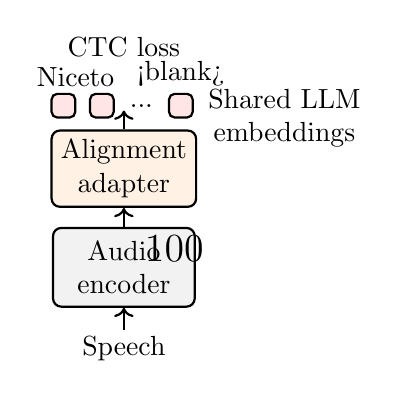
\begin{tikzpicture} [scale=0.8]
        \node(ae) at (0,0) [rectangle, draw=black, fill=gray!10, rounded corners=3pt, thick, minimum width=1.8cm,minimum height=1cm,align=center] {Audio\\encoder};
        \node(freeze) at ([xshift=0.8cm,yshift=0.3cm]ae.center) [rectangle, align=center] {\Large{\ding{100}}};
        \node(fb) at ([yshift=-0.3cm]ae.south) [rectangle, align=center,anchor=north] {Speech};
        \node(aa) at ([yshift=0.3cm]ae.north) [rectangle, draw=black, fill=orange!10, rounded corners=3pt, thick, minimum width=1.8cm,minimum height=0.5cm,align=center,anchor=south] {Alignment\\adapter};
        
        \node(f1) at ([yshift=1.0cm]aa.west) [rectangle, draw=black, fill=red!10, rounded corners=2pt, thick, minimum width=0.3cm, minimum height=0.3cm,align=center,anchor=west] {};
        \node(f2) at ([xshift=0.2cm]f1.east) [rectangle, draw=black, fill=red!10, rounded corners=2pt, thick, minimum width=0.3cm, minimum height=0.3cm,align=center,anchor=west] {};
        \node(f3) at ([xshift=0.075cm]f2.east) [rectangle, draw=white,  thick, align=center,anchor=west] {...};
        \node(f4) at ([xshift=0.075cm]f3.east) [rectangle, draw=black, fill=red!10, rounded corners=2pt, thick, minimum width=0.3cm, minimum height=0.3cm,align=center,anchor=west] {};
        \node(t1) at ([yshift=-0.05cm]f1.north) [rectangle, align=center,anchor=south] {Nice};
        \node(t2) at ([yshift=-0.05cm]f2.north) [rectangle, align=center,anchor=south] {to};
        \node(t4) at ([yshift=-0.05cm]f4.north) [rectangle, align=center,anchor=south] {<blank>};
        \node(se) at ([xshift=0.075cm,yshift=-0.2cm]f4.east) [rectangle, align=center,anchor=west] {Shared LLM\\embeddings};
        \node(ctc) at ([yshift=1.0cm]aa.north) [rectangle, rounded corners=3pt, thick, align=center,anchor=south] {CTC loss};

        
        \draw[->,thick]([yshift=-0.05cm]fb.north)--(ae.south);
        \draw[->,thick](ae.north)--(aa.south);
        \draw[->,thick](aa.north)--([yshift=0.3cm]aa.north);

        
      \end{tikzpicture}
    \end{minipage}
    }
    \subfigure[Shrinking stage]{
    \begin{minipage}[t]{0.45\linewidth}
    \centering
    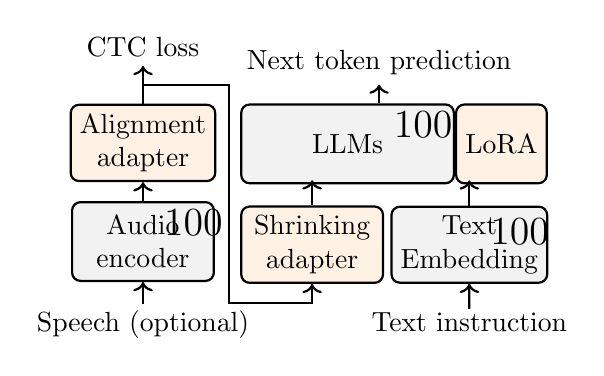
\begin{tikzpicture} [scale=0.8]
        \node(ae) at (0,0) [rectangle, draw=black, fill=gray!10, rounded corners=3pt, thick, minimum width=1.8cm,minimum height=1cm,align=center] {Audio\\encoder};
        \node(freeze) at ([xshift=0.8cm,yshift=0.3cm]ae.center) [rectangle, align=center] {\Large{\ding{100}}};
        \node(fb) at ([yshift=-0.3cm]ae.south) [rectangle, align=center,anchor=north] {Speech (optional)};
        \node(aa) at ([yshift=0.3cm]ae.north) [rectangle, draw=black, fill=orange!10, rounded corners=3pt, thick, minimum width=1.8cm,minimum height=0.5cm,align=center,anchor=south] {Alignment\\adapter};
        \node(ctc) at ([yshift=0.6cm]aa.north) [rectangle,align=center,anchor=south] {CTC loss};
        \node(sa) at ([xshift=0.4cm,yshift=-0.05cm]ae.east) [rectangle, draw=black, fill=orange!10, rounded corners=3pt, thick, minimum width=1.8cm,minimum height=0.5cm,align=center,anchor=west] {Shrinking\\adapter};
        \node(llm) at ([yshift=1.6cm]sa.west) [rectangle, draw=black, fill=gray!10, rounded corners=3pt, thick, minimum width=2.7cm,minimum height=1.0cm,align=center,anchor=west] {LLMs};
        \node(lora) at (llm.east) [rectangle, draw=black, fill=orange!10, rounded corners=3pt, thick, minimum width=1.0cm,minimum height=1.0cm,align=center,anchor=west] {LoRA};
        \node(te) at ([xshift=0.1cm]sa.east) [rectangle, draw=black, fill=gray!10, rounded corners=3pt, thick, minimum width=1.8cm,minimum height=0.5cm,align=center,anchor=west] {Text\\Embedding};
        \node(freeze3) at ([xshift=0.8cm,yshift=0.2cm]te.center) [rectangle, align=center] {\Large{\ding{100}}};
        \node(ti) at ([yshift=-0.3cm]te.south) [rectangle, align=center,anchor=north] {Text instruction};
        \node(freeze2) at ([xshift=1.2cm,yshift=0.3cm]llm.center) [rectangle, align=center] {\Large{\ding{100}}};
        \node(loss) at ([xshift=0.5cm, yshift=0.3cm]llm.north) [rectangle, align=center,anchor=south] {Next token prediction};

        
        \draw[->,thick]([yshift=-0.05cm]fb.north)--(ae.south);
        \draw[->,thick](ae.north)--(aa.south);
        \draw[->,thick](aa.north)--(ctc.south);
        \draw[->,thick](sa.north)--([yshift=0.4cm]sa.north);
        \draw[->,thick](te.north)--([yshift=0.4cm]te.north);
        \draw[->,thick]([yshift=-0.3cm]loss.south)--(loss.south);
        \draw[->,thick]([yshift=-0.1cm]ti.north)--(te.south);

        \draw[->,thick](aa.north)--([yshift=0.3cm]aa.north)--([xshift=0.2cm, yshift=0.3cm]aa.north -| aa.east)--([xshift=0.2cm, yshift=-0.3cm]sa.south -| aa.east)--([yshift=-0.3cm]sa.south)--(sa.south);
      \end{tikzpicture}
    \end{minipage}
    }
    \subfigure[SFT stage]{
    \begin{minipage}[t]{0.20\linewidth}
    \centering
    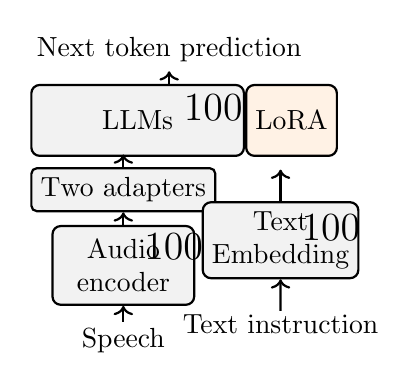
\begin{tikzpicture} [scale=0.8]
        \node(ae) at (0,0) [rectangle, draw=black, fill=gray!10, rounded corners=3pt, thick, minimum width=1.8cm,minimum height=1cm,align=center] {Audio\\encoder};
        \node(freeze) at ([xshift=0.8cm,yshift=0.3cm]ae.center) [rectangle, align=center] {\Large{\ding{100}}};
        \node(fb) at ([yshift=-0.2cm]ae.south) [rectangle, align=center,anchor=north] {Speech};
        \node(aa) at ([yshift=0.2cm]ae.north) [rectangle, draw=black, fill=gray!10, rounded corners=2pt, thick, minimum width=1.8cm,minimum height=0.5cm,align=center,anchor=south] {Two adapters};
        
        \node(llm) at ([yshift=1.1cm]aa.west) [rectangle, draw=black, fill=gray!10, rounded corners=3pt, thick, minimum width=2.7cm,minimum height=0.9cm,align=center,anchor=west] {LLMs};
        \node(lora) at (llm.east) [rectangle, draw=black, fill=orange!10, rounded corners=3pt, thick, minimum width=0.9cm,minimum height=0.9cm,align=center,anchor=west] {LoRA};
        \node(te) at ([xshift=0.1cm,yshift=0.4cm]ae.east) [rectangle, draw=black, fill=gray!10, rounded corners=3pt, thick, minimum width=1.8cm,minimum height=0.5cm,align=center,anchor=west] {Text\\Embedding};
        \node(freeze3) at ([xshift=0.8cm,yshift=0.2cm]te.center) [rectangle, align=center] {\Large{\ding{100}}};
        \node(ti) at ([yshift=-0.4cm]te.south) [rectangle, align=center,anchor=north] {Text instruction};
        \node(freeze2) at ([xshift=1.2cm,yshift=0.2cm]llm.center) [rectangle, align=center] {\Large{\ding{100}}};
        \node(loss) at ([xshift=0.5cm, yshift=0.2cm]llm.north) [rectangle, align=center,anchor=south] {Next token prediction};
       
        \draw[->,thick]([yshift=-0.05cm]fb.north)--(ae.south);
        \draw[->,thick](ae.north)--(aa.south);
        \draw[->,thick](aa.north)--([yshift=0.2cm]aa.north);
        \draw[->,thick](te.north)--([yshift=0.5cm]te.north);
        \draw[->,thick]([yshift=-0.2cm]loss.south)--(loss.south);
        \draw[->,thick]([yshift=-0.1cm]ti.north)--(te.south);
        
      \end{tikzpicture}
    \end{minipage}
    }
      \caption{Training progress of Soundwave. The gray modules are frozen while the orange modules are updated.}
      \label{architecture}
  \end{figure*}

  



\section{Fine-Tuning Experiments}
This section validates that our dataset can enhance the GUI grounding capabilities of VLMs and that the proposed functionality grounding and referring are effective fine-tuning tasks.
\subsection{Experimental Settings}
\noindent\textbf{Evaluation Benchmarks} We base our evaluation on the UI grounding benchmarks for various scenarios: \textbf{FuncPred} is the test split from our collected functionality dataset. This benchmark requires a model to locate the element specified by its functionality description. \textbf{ScreenSpot}~\citep{cheng2024seeclick} is a benchmark comprising test samples on mobile, desktop, and web platforms. It requires the model to locate elements based on short instructions. \textbf{RefExp}~\citep{Bai2021UIBertLG} is to locate elements given crowd-sourced referring expressions. \textbf{VisualWebBench (VWB)}~\citep{liu2024visualwebbench} is a comprehensive multi-modal benchmark assessing the understanding capabilities of VLMs in web scenarios. We select the element and action grounding tasks from this benchmark. To better align with high-level semantic instructions for potential agent requirements and avoid redundancy evaluation with ScreenSpot, we use ChatGPT to expand the OCR text descriptions in the original task instructions, such as \textit{Abu Garcia College Fishing} into functionality descriptions like \textit{This element is used to register for the Abu Garcia College Fishing event}.
\textbf{MOTIF}~\citep{Burns2022ADF} requires an agent to complete a natural language command in mobile Apps.
For all of these benchmarks, we report the grounding accuracy (\%): $\text { Acc }= \sum_{i=1}^N \mathbf{1}\left(\text {pred}_i \text { inside GT } \text {bbox}_i\right) / N \times 100 $ where $\mathbf{1}$ is an indicator function and $N$ is the number of test samples. This formula denotes the percentage of samples with the predicted points lying within the bounding boxes of the target elements.

\noindent\textbf{Training Details}
We select Qwen-VL-10B~\citep{bai2023qwen} and SliME-8B~\citep{slime} as the base models and fine-tune them on 25k, 125k, and 702k samples of the AutoGUI training data to investigate how the AutoGUI data enhances the UI grounding capabilities of the VLMs. The models are fine-tuned on 8 A100 GPUs for one epoch. We follow SeeClick~\citep{cheng2024seeclick} to fine-tune Qwen-VL with LoRA~\citep{hu2022lora} and follow the recipe of SliME~\citep{slime} to fine-tune it with only the visual encoder frozen (More details in Sec.~\ref{sec:supp:impl details}).

\noindent\textbf{Compared VLMs}
We compare with both general-purpose VLMs (i.e., LLaVA series~\citep{liu2023llava,liu2024llavanext}, SliME~\citep{slime}, and Qwen-VL~\citep{bai2023qwen}) and UI-oriented ones (i.e., Qwen2-VL~\citep{qwen2vl}, SeeClick~\citep{cheng2024seeclick}, CogAgent~\citep{hong2023cogagent}). SeeClick finetunes Qwen-VL with around 1 million data combining various data sources, including a large proportion of human-annotated UI grounding/referring samples. CogAgent is trained with a huge amount of text recognition, visual grounding, UI understanding, and publicly available text-image datasets, such as LAION-2B~\citep{LAION5B}. During the evaluation, we manually craft grounding prompts suitable for these VLMs.
\subsection{Experimental Results and Analysis}
\begin{table}[]
\scriptsize
\centering
\caption{\textbf{Element grounding accuracy on the used benchmarks.} We compare the base models fine-tuned with our AutoGUI data and representative open-source VLMs. The results show that the two base models (i.e. Qwen-VL and SliME-8B) obtain significant performance gains over the benchmarks after being fine-tuned with AutoGUI data. Moreover, increasing the AutoGUI data size consistently improves grounding accuracy, demonstrating notable scaling effects. $\dag$ means the metric value is borrowed from the benchmark paper. $*$ means using additional SeeClick training data.}
\label{tab:eval results}
\begin{tabular}{@{}cccccccccc@{}}
\toprule
Type & Model    & Size    & FuncPred & VWB EG & VWB AG & MoTIF & RefExp & ScreenSpot  \\ \midrule
\multirow{5}{*}{General} & LLaVA-1.5~\citep{liu2023llava} & 7B & 3.2      &        12.1$^{\dag}$        &     13.6$^{\dag}$           &  7.2   &  4.2 & 5.0 & \\
 & LLaVA-1.5~\citep{liu2023llava} & 13B & 5.8      &           16.7     &        9.7        &   12.3 &  20.3   & 11.2 &  \\
 & LLaVA-1.6~\citep{liu2024llavanext} & 34B &  4.4      &      19.9          &    17.0            &   7.0 &  29.1  & 10.3 &  \\
 & SliME~\citep{slime} & 8B &  3.2  &   6.1       &     4.9     & 7.0  &  8.3  &  13.0  \\ 

 & Qwen-VL~\citep{bai2023qwen} & 10B &  3.0     &      1.7          &      3.9          &    7.8 &  8.0  & 5.2$^{\dag}$   \\ 
 \midrule
\multirow{3}{*}{UI-VLM} &  Qwen2-VL~\citep{bai2023qwen}  & 7B     &     7.8       &    3.9        &  3.9  &  16.7 & 32.4 & 26.1    \\
 & CogAgent~\citep{hong2023cogagent} & 18B    &  29.3   &    \underline{55.7}      &    \textbf{59.2}      & \textbf{24.7}   & 35.0 &  47.4$^{\dag}$  \\
 & SeeClick~\citep{cheng2024seeclick} & 10B    &    19.8     &    39.2           &     27.2           & 11.1  &  \textbf{58.1}  & \underline{53.4}$^{\dag}$ \\ 
\midrule
\multirow{4}{*}{Finetuned} &  Qwen-VL-AutoGUI25k & 10B      &    14.2     &      12.8         &    12.6           &   10.8    &  12.0 & 19.0    \\
 & Qwen-VL-AutoGUI125k  & 10B       &     25.5     &      23.2         &        29.1       &    11.5   &  14.9 & 32.0     \\ 
 & Qwen-VL-AutoGUI702k  & 10B       &   43.1   &    38.0       &     32.0    &  15.5  & 23.9 &    38.4   \\
& Qwen-VL-AutoGUI702k$^*$   & 10B     &  \underline{50.0}  &    \textbf{56.2}    &  \underline{45.6}  & \underline{21.0} & \underline{51.5} & \textbf{54.2}      \\
\midrule
\multirow{3}{*}{Finetuned} & SliME-AutoGUI25k  & 8B     &   28.0   &     14.0      &      10.6      &  14.3   & 18.4 & 27.2   \\
 & SliME-AutoGUI125k   & 8B      &   39.9    &  22.0   &     12.0       &  17.8  & 22.1 &  35.0     \\
 & SliME-AutoGUI702k   & 8B      &     \textbf{62.6}   &       25.4        &     13.6          &   20.6    & 26.7 & 44.0 &          \\
\bottomrule
\end{tabular}
\end{table}
\vspace{-2mm}


\noindent\textbf{A) AutoGUI functionality annotations effectively enhance VLMs' UI grounding capabilities and achieve scaling effects.} We endeavor to show that the element functionality data autonomously collected by AutoGUI contributes to high grounding accuracy. The results in Tab.~\ref{tab:eval results} demonstrate that on all benchmarks the two base models achieve progressively rising grounding accuracy as the functionality data size scales from 25k to 702k, with SliME-8B's accuracy increasing from merely \textbf{3.2} and \textbf{13.0} to \textbf{62.6} and \textbf{44.0} on FuncPred and ScreenSpot, respectively. This increase is visualized in Fig.~\ref{fig:funcpred scaling success} showing that increasing AutoGUI data amount leads to more precise localization performance.

After fine-tuning with AutoGUI 702k data, the two base models surpass SeeClick, the strong UI-oriented VLM on FuncPred and MOTIF. We notice that the base models lag behind SeeClick and CogAgent on ScreenSpot and RefExp, as the two benchmarks contain test samples whose UIs cannot be easily recorded (e.g., Apple devices and Desktop software) as training data, causing a domain gap. Nevertheless, SliME-8B still exhibits noticeable performance improvements on ScreenSpot and RefExp when scaling up the AutoGUI data, suggesting that the AutoGUI data helps to enhance grounding accuracy on the out-of-domain tasks.

To further unleash the potential of the AutoGUI data, the base model, Qwen-VL, is finetuned with the combination of the AutoGUI and SeeClick UI-grounding data. This model becomes the new state-of-the-art on FuncPred, ScreenSpot, and VWB EG, surpassing SeeClick and CogAgent. This result suggests that our AutoGUI data can be mixed with existing UI grounding training data to foster better UI grounding capabilities.

In summary, our functionality data can endow a general VLM with stronger UI grounding ability and exhibit clear scaling effects as the data size increases.


\begin{table}[]
\centering
\footnotesize
\caption{\textbf{Comparing the AutoGUI functionality annotation type with existing types}. Qwen-VL is fine-tuned with the three annotation types. The results show that our functionality data leads to superior grounding accuracy compared with the naive element-HTML data and the condensed functionality annotations.}
\label{tab:ablation}
\begin{tabular}{@{}ccccc@{}}
\toprule
Data Size             & Variant          & FuncPred & RefExp & ScreenSpot \\ \midrule
\multirow{3}{*}{25k}  & w/ Elem-HTML data     &  5.3      &  4.5   &    5.7     \\
                      & w/ Condensed Func. Anno.     &  3.8   &  3.0  &   4.8      \\
                      & w/ Func. Anno. (Ours full)         &    \textbf{21.1}    &   \textbf{10.0}   &   \textbf{16.4}    \\ \midrule
\multirow{3}{*}{125k} & w/ Elem-HTML data     &  15.5   &  7.8  &   17.0      \\
                      & w/ Condensed Func. Anno.     &  14.1   &  11.7  &   23.8      \\
                      & w/ Func. Anno. (Ours full)         &  \textbf{24.6}   &  \textbf{12.7}  &   \textbf{27.0}    \\ \bottomrule
\end{tabular}
\end{table}



\noindent\textbf{B) Our functionality annotations are effective for enhancing UI grounding capabilities.} To assess the effectiveness of functionality annotations, we compare this annotation type with two existing types: 1) \textbf{Naive element-HTML pairs}, which are directly obtained from the UI source code~\citep{hong2023cogagent} and associate HTML code with elements in specified areas of a screenshot. Examples are shown in Fig.~\ref{fig: functionality vs others}. To create these pairs, we replace the functionality annotations with the corresponding HTML code snippets recorded during trajectory collection. 2) \textbf{Brief functionality descriptions} that are generated by prompting GPT-4o-mini\footnote{https://openai.com/index/gpt-4o-mini-advancing-cost-efficient-intelligence/} to condense the AutoGUI functionality annotations. For example, a full description such as \textit{`This element provides access to a documentation category, allowing users to explore relevant information and guides'} is shortened to \textit{`Documentation category access'}.

After experimenting with Qwen-VL~\citep{bai2023qwen} at the 25k and 125k scales, the results in Tab.~\ref{tab:ablation} show that fine-tuning with the complete functionality annotations is superior to the other two types. Notably, our functionality annotation type yields the largest gain on the challenging FuncPred benchmark that emphasizes contextual functionality grounding. In contrast, the Elem-HTML type performs poorly due to the noise inherent in HTML code (e.g., numerous redundant tags), which reduces fine-tuning efficiency. The condensed functionality annotations are inferior, as the consensing loses details necessary for fine-grained UI understanding. In summary, the AutoGUI functionality annotations provide a clear advantage in enhancing UI grounding capabilities.


\subsection{Failure Case Analysis}
After analyzing the grounding failure cases, we identified several failure patterns in the fine-tuned models: a) difficulty in accurately locating small elements; b) challenges in distinguishing between similar but incorrect elements; and c) issues with recognizing icons that have uncommon shapes. Please refer to Sec.~\ref{sec:supp:case analysis} for details.



\section{Discussion}

This study presents PathFinder, a multi-modal, multi-agent AI framework designed to emulate the multi-scale, iterative diagnostic approach of expert pathologists for histopathology whole slide images (WSIs). By integrating Triage, Navigation, Description, and Diagnosis Agents, PathFinder collaboratively gathers evidence to deliver accurate, interpretable diagnoses with natural language explanations. Notably, it surpasses state-of-the-art methods and the average performance of human experts in melanoma diagnosis, setting a new benchmark in AI-driven pathology.

PathFinder has the potential to accelerate diagnostic workflows, reducing the reliance on manual examination and enabling timely patient care in clinical settings. Its natural language descriptions provide interpretability, facilitating the validation of AI-generated diagnoses by pathologists. Moreover, its integration of vision-language models (VLMs) and large language models (LLMs) highlights the promise of multi-modal AI in delivering scalable, specialized diagnostic tools that could improve access to pathology expertise.

\noindent\textbf{Limitations.} Despite its strengths, PathFinder has limitations. The framework relies on pre-existing datasets and significant computational resources, posing challenges in resource-constrained environments. Additionally, the complexity of the Navigation Agent’s decision-making process and occasional hallucinations by the Description Agent could affect transparency and accuracy of the decision-making process. Future work should address these issues by enhancing dataset diversity, computational efficiency, and patch selection strategies, further advancing PathFinder's potential as a transformative tool in AI-assisted pathology.


\section*{Acknowledgments}
This work was financially supported by the Bavarian State Ministry of Education, Science and the Arts, the Alan Turing Institute’s studentship scheme, and the Engineering and Physical Sciences Research Council [EP/S023917/1].

\section*{Impact Statement}
This paper presents work whose goal is to advance the field of Machine Learning. 
There are many potential societal consequences of our work, none which we feel must be specifically highlighted here. We further emphasize that the health-related causal graph serves as a simplified illustrative example and, as such, carries no ethical concerns.

\bibliography{references}
\bibliographystyle{icml2025}

\newpage
\appendix
\onecolumn
\section{Decomposition of \textsc{mo-cbo} Problems}\label{appendix:mo_cbo_decomposition}

Recall the definition of the local \textsc{mo-cbo} problems.

\textbf{Definition \ref{def:local_mocbo_problem} \textnormal{(Local \textsc{mo-cbo} problem)}.}
Let $\textbf{X}_s \in \mathbb{P}(\mathbf{X})$ be an intervention set. Then, the multi-objective optimization problem defined by the objective functions $\mu_i(\mathbf{X}_s,\ \cdot \ ): \mathcal{D}(\mathbf{X}_s) \rightarrow \mathbb{R}$, $\mathbf{x}_s \mapsto \mu(\mathbf{X}_s,\mathbf{x}_s)$, $1 \leq i \leq m$, is called \textit{local \textsc{mo-cbo} problem w.r.t. $\mathbf{X}_s$}.

For the local \textsc{mo-cbo} problem w.r.t. $\mathbf{X}_s \in \mathbb{P}(\mathbf{X})$, we denote its Pareto set as $\mathcal{P}_s^{\textsf{l}}(\mathbf{X}_s)$ and the associated Pareto front as $\mathcal{P}_f^{\textsf{l}}(\mathbf{X}_s)$. 

\textbf{Proposition \ref{prop:mo_cbo.decomposition}.} \textit{Given $\langle \mathcal{G}, \mathbf{Y},\mathbf{X}, \mathbf{C} \rangle$, let $\mathcal{S} \subseteq \mathbb{P}(\mathbf{X})$ be a non-empty collection of intervention sets. Then, it holds}
\begin{equation}
    \mathcal{P}_f^{\textsf{c}}(\mathcal{S}) \subseteq \bigcup_{s=1}^{|\mathcal{S}|} \mathcal{P}_f^{\textsf{l}}(\mathbf{X}_s).
\end{equation}

\begin{proof}
    Assume for contradiction that $\mathcal{P}_f^{\textsf{c}}(\mathcal{S}) \not\subseteq \bigcup_{s=1}^{|\mathcal{S}|} \mathcal{P}_f^{\textsf{l}}(\mathbf{X}_s)$. Then, there exists some $\mathbf{z} \in \mathbb{R}^m$ such that $\mathbf{z} \in \mathcal{P}_f^{\textsf{c}}(\mathcal{S})$ and $\mathbf{z} \not\in \mathcal{P}_f^{\textsf{l}}(\mathbf{X}_{s})$ for all $s = 1, \dots, |\mathcal{S}|$. For some intervention set $\mathbf{X}_{s}' \in \mathcal{S}$ and intervention value $\mathbf{x}_s' \in \mathcal{D}(\mathbf{X}_s')$, it holds $\mathbf{z} = (\mu_1(\mathbf{X}_s',\mathbf{x}_s'),\dots,\mu_m(\mathbf{X}_s',\mathbf{x}_s'))$. Let $\mathcal{P}_s^{\textsf{l}}(\mathbf{X}_1),\dots,\mathcal{P}_s^{\textsf{l}}(\mathbf{X}_{|\mathcal{S}|})$ be the Pareto sets of the associated local \textsc{mo-cbo} problems w.r.t. $\mathbf{X}_1,\dots,\mathbf{X}_{|\mathcal{S}|}$, respectively. Since $\mathbf{z} \not\in \mathcal{P}_f^{\textsf{l}}(\mathbf{X}_s')$, it follows $\mathbf{x}_s' \not\in \mathcal{P}_s^{\textsf{l}}(\mathbf{X}_s')$, i.e. $\mathbf{x}_s'$ is not Pareto-optimal in the local \textsc{mo-cbo} problem w.r.t. $\mathbf{X}_s'$. Thus, there exists another intervention value $\mathbf{x}_s'' \in \mathcal{D}(\mathbf
    {X}_s')$ such that $\mu_i(\mathbf{X}_s',\mathbf{x}_s') \geq \mu_i(\mathbf{X}_s',\mathbf{x}_s'')$ for all $i$ and $\mu_i(\mathbf{X}_s',\mathbf{x}_s') > \mu_i(\mathbf{X}_s',\mathbf{x}_s'')$ for at least one $1 \leq i \leq m$. In other words, the intervention set-value pair $(\mathbf{X}_s',\mathbf{x}_s')$ is not Pareto-optimal for $\mathcal{S}$ since it is dominated by $(\mathbf{X}_s',\mathbf{x}_s'')$. Therefore, $\mathbf{z} \not\in \mathcal{P}_f^{\textsf{c}}(\mathcal{S})$ which is a contradiction.
\end{proof}

\section{Reducing the Search Space}\label{appendix:search_space_reduction}
\citet{NEURIPS2018_c0a271bc} leverage the graph topology of an \textsc{scm} to identify intervention sets that are redundant to consider in any optimisation scheme. Their formalism exploits the rules of do-calculus to identify invariances and partial-orders among intervention sets, in order to obtain those sets that could potentially yield optimal outcomes for a given graph. To take advantage of their ideas for this paper, the relevant concepts and their theoretical properties must be extended to accommodate multi-target settings, which will be the focus of this section.

Let $\langle \mathbf{V}, \mathbf{U}, \mathbf{F}, P(\textbf{U}) \rangle$ denote an \textsc{scm} and $\mathcal{G}$ its associated acyclic graph that encodes the underlying causal mechanisms. Recall that we assume $\mathbf{C} = \varnothing$, i.e., there are no non-manipulative variables. In this section, we require the notation $\mathbb{E}_{P(\mathbf{W} | \text{do}(\mathbf{X}_s = \mathbf{x}_s))}[\mathbf{W}] := \mathbb{E}[\mathbf{W} | \text{do}(\mathbf{X}_s = \mathbf{x}_s)]$ for sets $\mathbf{X}_s \subseteq \mathbf{X}$, $\mathbf{W} \subseteq \mathbf{V}$.

\subsection{Equivalence of Intervention Sets}\label{subsec:causal_bandits_mis}

As a first step, we establish invariances within $\mathbb{P}(\mathbf{X})$ in regards to the effects of intervention sets on the target variables. Recall the following definition from the main part of the paper.

\textbf{Definition \ref{def:causal_bandits.mis} \textnormal{(Minimal intervention set)}.} A set $\mathbf{X}_s \in \mathbb{P}(\mathbf{X})$ is called a \textit{minimal intervention set} if, for every \textsc{scm} conforming to $\mathcal{G}$, there exists no subset $\mathbf{X}_s' \subset \mathbf{X}_s$ such that for all $\mathbf{x}_s \in \mathcal{D}(\mathbf{X}_s)$ it holds $\mu(\mathbf{X_s},\mathbf{x}_s) = \mu(\mathbf{X}_s',\mathbf{x}_s[\mathbf{X}_s'])$, for all $1 \leq i \leq m$.

We denote the set of minimal intervention sets with $\mathbb{M}_{\mathcal{G},\mathbf{Y}}$. In other words, no subset of a minimal intervention set can achieve the same expected outcome on $\mathbf{Y}$. Intervention sets, that are not \textit{minimal} in the sense of Definition \ref{def:causal_bandits.mis}, are redundant to consider in any optimization task. 

\textbf{Proposition \ref{prop:causal_bandits.mis}.} 
\textit{$\mathbf{X}_s \in \mathbb{P}(\mathbf{X})$ is a minimal intervention set if and only if it holds $\mathbf{X}_s \subseteq \textnormal{an}(\mathbf{Y})_{\mathcal{G}_{\overline{\mathbf{X}}_s}}$.}

\begin{proof}
    (If) Let $\mathbf{x}_s \in \mathcal{D}(\mathbf{X}_s)$ be any intervention value. Assume that there is a subset $\mathbf{X}_s' \subset \mathbf{X}_s$ such that $\mathbb{E}[Y_i | \text{do}(\mathbf{X}_s = \mathbf{x}_s)] = \mathbb{E}[Y_i | \text{do}(\mathbf{X}_s' = \mathbf{x}_s[\mathbf{X}_s'])]$ for all $1 \leq i \leq m$. Consider an \textsc{scm} with real-valued variables where each $V \in \mathbf{V}$ is associated with its own binary exogenous variable $U_V$ with $P(U_V=1)=0.5$. Let the function of an endogenous variable be the sum of values of its parents. For the sake of contradiction, assume $\mathbf{X}_s \subseteq \text{an}(\mathbf{Y})_{\mathcal{G}_{\overline{\mathbf{X}}_s}}$. Then, there exists a directed path from $\mathbf{X}_s \backslash \mathbf{X}_s'$ to some $Y_i$ without passing $\mathbf{X}_s'$. Hence, setting $\mathbf{W} = \mathbf{X}_s \backslash \mathbf{X}_s'$ to the values \mbox{$\mathbf{w} = \mathbb{E}[\mathbf{W} | \text{do}(\mathbf{X}_s' = \mathbf{x}_s[\mathbf{X}_s'])] + 1$} yields \mbox{$\mathbb{E}[Y_i | \text{do}(\mathbf{W} = \mathbf{w}, \mathbf{X}_s' = \mathbf{x}_s[\mathbf{X}_s'])] >$} \mbox{$\mathbb{E}[Y_i | \text{do}(\mathbf{X}_s' = \mathbf{x}_s[\mathbf{X}_s'])]$}, contradicting the assumption.
    
    (Only if) Assume that $\mathbf{X}_s \not\subseteq \text{an}(\mathbf{Y})_{\mathcal{G}_{\overline{\mathbf{X}}_s}}$. Then, for $\mathbf{X}_s' = \mathbf{X}_s \cap \text{an}(\mathbf{Y})_{\mathcal{G}_{\overline{\mathbf{X}}_s}}$ it holds $\mathbf{X}_s' \subset \mathbf{X}_s$ and by the third rule of do-calculus, for every $\mathbf{x}_s \in \mathcal{D}(\mathbf{X}_s)$ it holds $\mathbb{E}[Y_i | \text{do}(\mathbf{X}_s = \mathbf{x}_s)] = \mathbb{E}[Y_i | \text{do}(\mathbf{X}_s' = \mathbf{x}_s[\mathbf{X}_s'])]$, $1 \leq i \leq m$. This is a contradiction because $\mathbf{X}_s$ was assumed to be a minimal intervention set.
\end{proof}

\subsection{Partial-Orders among Intervention Sets}\label{subsec:causal_bandits_pomis}

Recall the definition of possibly Pareto-optimal minimal intervention sets.

\textbf{Definition \ref{def:causal_bandits.pomis} \textnormal{(Possibly Pareto-optimal minimal intervention set)}.}
    A set $\mathbf{X}_s \in \mathbb{M}_{\mathcal{G},\mathbf{Y}}$ is called \textit{possibly Pareto-optimal} if, for at least one \textsc{scm} conforming to $\mathcal{G}$, there exists $\mathbf{x}_s \in \mathcal{D}(\mathbf{X}_s)$ such that $(\mathbf{X}_s,\mathbf{x}_s)$ is Pareto-optimal for $\mathbb{P}(\mathbf{X})$, and for no $\mathbf{X}_s' \in \mathbb{M}_{\mathcal{G},\mathbf{Y}} \backslash \mathbf{X}_s, \mathbf{x}_s' \in \mathcal{D}(\mathbf{X}_s')$ it holds $\mu(\mathbf{X}_s',\mathbf{x}_s') \leq \mu(\mathbf{X}_s,\mathbf{x}_s)$, for all $1\leq i \leq m$.

Characterizing such sets is the aim of this section. For simplicity, we first consider the special case in which $\mathcal{G}$ exhibits no unobserved confounders between $Y_i$ and any of its ancestors. 

\textbf{Proposition \ref{prop:causal_bandits.pomis_no_confounders}.} \textit{If no $Y_i$ is confounded with $\textnormal{an}(Y_i)_{\mathcal{G}}$ via unobserved confounders, then $\textnormal{pa}(\mathbf{Y})_{\mathcal{G}}$ is the only possibly Pareto-optimal minimal intervention set.}


\begin{proof}\label{proof:causal_bandits.pomis_no_confounders}
    Let $\mathbf{X}_s = \text{pa}(\mathbf{Y})_{\mathcal{G}}$, and let $\text{pa}(\mathbf{Y})_{\mathcal{G}} \neq \mathbf{X}_s'$ be another minimal intervention set with $\mathbf{x}_s' \in \mathcal{D}(\mathbf{X}_s')$. Define $\mathbf{Z}=\mathbf{X}_s \backslash (\mathbf{X}_s' \cap \mathbf{X}_s)$ and $\mathbf{W}=\mathbf{X}_s' \backslash (\mathbf{X}_s' \cap \mathbf{X}_s)$. Moreover, we choose an intervention value $\mathbf{x}_s^* \in \mathcal{D}(\mathbf{X}_s)$ such that it dominates $\mathbf{x}_s \in \mathcal{D}(\mathbf{X}_s)$ which is given by $\mathbf{x}_s[\mathbf{X}_s']=\mathbf{x}_s'[\mathbf{X}_s]$ and $\mathbf{x}_s[\mathbf{Z}] = \mathbb{E}[\mathbf{Z} | \text{do}(\mathbf{X}_s' = \mathbf{x}_s')]$. If $\mathbf{x}_s$ is non-dominated, define $\mathbf{x}_s^*=\mathbf{x}_s$. Then, for all $i=1,\dots,m$ it holds
    \begin{align}
        \mathbb{E} [Y_i | \text{do}(\mathbf{X}_s = \mathbf{x}_s^*)] & = \mathbb{E}[Y_i | \text{do}(\mathbf{X}_s \cap \mathbf{X}_s' = \mathbf{x}_s^*[\mathbf{X}_s'], \mathbf{Z} = \mathbf{x}_s^*[\mathbf{Z}])] \\
        &\leq \mathbb{E}[Y_i | \text{do}(\mathbf{X}_s \cap \mathbf{X}_s' = \mathbf{x}_s[\mathbf{X}_s'], \mathbf{Z} = \mathbf{x}_s[\mathbf{Z}])] \\
        & = \mathbb{E}[Y_i | \text{do}(\mathbf{X}_s \cap \mathbf{X}_s' = \mathbf{x}_s[\mathbf{X}_s'], \mathbf{Z} = \mathbf{x}_s[\mathbf{Z}], \mathbf{W}=\mathbf{x}_s'[\mathbf{W}])] \\
        & = \mathbb{E}[Y_i | \text{do}(\mathbf{X}_s \cap \mathbf{X}_s' = \mathbf{x}_s[\mathbf{X}_s'], \mathbf{W}=\mathbf{x}_s'[\mathbf{W}]), \mathbf{Z} = \mathbf{x}_s[\mathbf{Z}]] \\
        &= \mathbb{E}[Y_i | \text{do}(\mathbf{X}_s \cap \mathbf{X}_s' = \mathbf{x}_s[\mathbf{X}_s'], \mathbf{W}=\mathbf{x}_s'[\mathbf{W}])] \displaybreak[1] \\
        &= \mathbb{E}[Y_i | \text{do}(\mathbf{X}_s' = \mathbf{x}_s')],
    \end{align}
    where the inequality holds because $\mathbf{x}_s$ (weakly) dominates $\mathbf{x}_s^*$. Note that the second and third equalities are derived through the third and second rules of do-calculus, respectively. The second rule of do-calculus assumes that $Y_i$ is not confounded with $\text{an}(Y_i)_{\mathcal{G}}$ via unobserved confounders. For $\mathbf{X}_s = \text{pa}(\mathbf{Y})_{\mathcal{G}}$, it is possible to construct an \textsc{scm}, conforming to $\mathcal{G}$, such that strict inequality holds for some $Y_i$, see the proof of \autoref{prop:causal_bandits_IB}. This shows that $\text{pa}(\mathbf{Y})_{\mathcal{G}}$ is the only possibly Pareto-optimal minimal intervention set.
\end{proof}

We continue and study the more general case where unobserved confounders can be present between $Y_i$ and any of its ancestors. For this intent, we extend two existing concepts, called \textit{minimal unobserved-confounders’ territory} and \textit{interventional border} \citep{NEURIPS2018_c0a271bc}, to the multi-objective setting. Using these notions, we derive results which can fully characterize possibly Pareto-optimal minimal intervention sets in the aforementioned scenario.

\textbf{Definition \ref{def:mo_cbo.uc_territory} \textnormal{(Minimal unobserved confounders' territory)}.}
Let $\mathcal{H}=\mathcal{G}[\text{An}(\mathbf{Y})_{\mathcal{G}}]$. A set of variables $\mathbf{T}$ in $\mathcal{H}$, with $\mathbf{Y} \subseteq \mathbf{T}$, is called a \textit{UC-territory} for $\mathcal{G}$ w.r.t. $\mathbf{Y}$ if $\text{De}(\mathbf{T})_{\mathcal{H}}=\mathbf{T}$ and $\text{CC}(\mathbf{T})_{\mathcal{H}} = \mathbf{T}$. The UC-territory $\mathbf{T}$ is said to be \textit{minimal}, denoted $\mathbf{T} = \text{MUCT}(\mathcal{G},\mathbf{Y})$, if no $\mathbf{T}' \subset \mathbf{T}$ is a UC-territory.

A minimal UC-territory for $\mathcal{G}$ w.r.t. $\mathbf{Y}$ can be constructed by extending a set of variables, starting from $\mathbf{Y}$, and iteratively updating the set with the c-component and descendants of the set. More intuitively, it is the minimal subset of $\text{An}(\mathbf{Y})_{\mathcal{G}}$ that is governed by unobserved confounders, where at least one target $Y_i$ is adjacent to an unobserved confounder.

\textbf{Definition \ref{def:mo_cbo.int_border} \textnormal{(Interventional border)}.}
Let $\mathbf{T}=\text{MUCT}(\mathcal{G},\mathbf{Y})$. Then, $\mathbf{B} = \text{pa}(\mathbf{T})_{\mathcal{G}} \backslash \mathbf{T}$ is called the \textit{interventional border} for $\mathcal{G}$ w.r.t. $\mathbf{Y}$, denoted as $\text{IB}(\mathcal{G},\mathbf{Y})$.

We have already described these concepts in the main part. Before connecting the notion of minimal UC-territory and interventional border to possibly Pareto-optimal minimal intervention sets, we require the following proposition:

\begin{proposition}
    \label{prop:causal_bandits.subsumption}
    Let $\mathbf{T}$ be a minimal UC-territory and $\mathbf{B}$ an interventional border for $\mathcal{G}$ w.r.t. $\mathbf{Y}$. Let $\mathbf{X}_s \subseteq \mathbf{X}$ be an intervention set and $\mathbf{S} = (\mathbf{T} \cap \mathbf{X}_s) \cup \mathbf{B}$. Then, for any $\mathbf{x}_s \in \mathcal{D}(\mathbf{X}_s)$ there exists $\mathbf{s} \in \mathcal{D}(\mathbf{S})$ such that $\mathbb{E}[Y_i | \textnormal{do}(\mathbf{S}=\mathbf{s})] \leq \mathbb{E}[Y_i | \textnormal{do}(\mathbf{X}_s=\mathbf{x}_s)]$, for all $i=1,\dots,m$.
\end{proposition}

\begin{proof}
    (Case $\mathbf{B} \subseteq \mathbf{X}_s$) Let $\mathbf{x}_s \in \mathcal{D}(\mathbf{X}_s)$ be an intervention value. Then, by the third rule of do-calculus, it holds $\mathbb{E}[Y_i | \text{do}(\mathbf{X}_s=\mathbf{x}_s)]=\mathbb{E}[Y_i | \text{do}(\mathbf{X}_s \cap (\mathbf{T} \cup \mathbf{B}) =\mathbf{x}_s[\mathbf{T} \cup \mathbf{B}])]$, $1 \leq i \leq m$. Since $\mathbf{X}_s \cap (\mathbf{T} \cup \mathbf{B}) = \mathbf{S}$, by setting $\mathbf{s} = \mathbf{x}_s[\mathbf{T} \cup \mathbf{B}]$, it follows $\mathbb{E}[Y_i | \text{do}(\mathbf{X}_s=\mathbf{x}_s)] = \mathbb{E}[Y_i | \text{do}(\mathbf{S}=\mathbf{s})]$.
    \vspace{0.2cm}\\
    (Case $\mathbf{B} \not\subseteq \mathbf{X}_s$) Let $\mathbf{x}_s \in \mathcal{D}(\mathbf{X}_s)$ be an intervention value. We define $\mathbf{B}' = \mathbf{S} \backslash (\mathbf{X}_s \cap \mathbf{S}) = \mathbf{S} \backslash (\mathbf{X}_s \cap (\mathbf{T} \cup \mathbf{B})) = \mathbf{B} \backslash (\mathbf{X}_s \cap \mathbf{B})$ and $\mathbf{W} = \mathbf{X}_s \backslash (\mathbf{X}_s \cap \mathbf{S}) = \mathbf{X}_s \backslash (\mathbf{X}_s \cap (\mathbf{T} \cup \mathbf{B}))$. Moreover, let $\mathbf{s}^* \in \mathcal{D}(\mathbf{S})$ such that it dominates $\mathbf{s} \in \mathcal{D}(\mathbf{S})$, which is given by $\mathbf{s}[\mathbf{B}'] = \mathbb{E}[\mathbf{B}' | \text{do}(\mathbf{X}_s=\mathbf{x}_s)]$ and $\mathbf{s}[\mathbf{X}_s] = \mathbf{x}_s[\mathbf{T} \cup \mathbf{B}]$. If $\mathbf{s}$ is non-dominated, we set $\mathbf{s}^* = \mathbf{s}$. Then, for all $i=1,\dots,m$ it holds
    \begin{align}
        \mathbb{E}[Y_i | \text{do}(\mathbf{S}=\mathbf{s}^*)] &= \mathbb{E}[Y_i | \text{do}(\mathbf{X}_s \cap (\mathbf{T} \cup \mathbf{B}) =\mathbf{s}^*[\mathbf{X}_s], \mathbf{B}'=\mathbf{s}^*[\mathbf{B}'])]\\
        & \leq \mathbb{E}[Y_i | \text{do}(\mathbf{X}_s \cap (\mathbf{T} \cup \mathbf{B}) =\mathbf{s}[\mathbf{X}_s], \mathbf{B}'=\mathbf{s}[\mathbf{B}'])] \\
        &= \mathbb{E}[Y_i | \text{do}(\mathbf{X}_s \cap (\mathbf{T} \cup \mathbf{B}) =\mathbf{s}[\mathbf{X}_s], \mathbf{B}'=\mathbf{s}[\mathbf{B}'], \mathbf{W}=\mathbf{x}_s[\mathbf{W}])]\\
        &=\mathbb{E}[Y_i | \text{do}(\mathbf{X}_s \cap (\mathbf{T} \cup \mathbf{B}) =\mathbf{s}[\mathbf{X}_s], \mathbf{W}=\mathbf{x}_s[\mathbf{W}]), \mathbf{B}'=\mathbf{s}[\mathbf{B}']]\\
        &= \mathbb{E}[Y_i | \text{do}(\mathbf{X}_s \cap (\mathbf{T} \cup \mathbf{B}) =\mathbf{s}[\mathbf{X}_s], \mathbf{W}=\mathbf{x}_s[\mathbf{W}])]\\
        &= \mathbb{E}[Y_i | \text{do}(\mathbf{X}_s=\mathbf{x}_s)],
    \end{align}
    where the inequality holds because $\mathbf{s}$ is (weakly) dominated by $\mathbf{s}^*$. Furthermore, the second and third equalities are derived through the third and second rules of do-calculus, respectively.
\end{proof}

The following proposition is a building block for characterizing possibly Pareto-optimal minimal intervention sets via interventional borders. The proof is similar to the one given by \citet{NEURIPS2018_c0a271bc} 

\begin{proposition}
    \label{prop:causal_bandits_IB}
    $\textnormal{IB}(\mathcal{G},\mathbf{Y})$ is a possibly Pareto-optimal minimal intervention set.
\end{proposition}

\begin{proof}
    The intuition of this proof is to construct an \textsc{scm}, conforming to $\mathcal{G}$, for which the single best strategy involves intervening on $\text{IB}(\mathcal{G},\mathbf{Y})$. Let $\mathbf{T}$ and $\mathbf{B}$ denote $\text{MUCT}(\mathcal{G},\mathbf{Y})$ and $\text{IB}(\mathcal{G},\mathbf{Y})$, respectively. Every exogenous variable in $\mathbf{U}$ shall be a binary variable with its domain being $\{ 0, 1\}$. Let $\oplus$ denote the exclusive-or function and $\bigvee$ the logical OR operator.
    \vspace{0.2cm}\\
    (Case $\mathbf{T} = \mathbf{Y}$) 
    In this case, $\mathbf{B}$ corresponds to the parents of $\mathbf{Y}$. Therefore, no target variable $Y_i$ is confounded with $\text{an}(Y_i)_{\mathcal{G}}$ via unobserved confounders. Define an \textsc{scm} such that
    \begin{itemize}
        \item Each endogenous variable $V \in \mathbf{V}$ is influenced by an exogenous variable $U_V \in \mathbf{V}$;
        \item $f_{Y_i} = \bigvee \mathbf{u}^{Y_i} \oplus \bigvee \mathbf{pa}_{Y_i}$ with $P(\mathbf{U}^{Y_i}=0) \approx 1$, for all $i=1,\dots,m$;
        \item $f_{X} = (\bigoplus \mathbf{u}^X) \oplus (\bigoplus \mathbf{pa}_X)$ for $X \in \mathbf{X}$ and $P(U = 0) = 0.5$ for every $U \in \mathbf{U} \backslash (\bigcup_{i=1}^m \mathbf{U}^{Y_i})$. 
    \end{itemize}
    By the third rule of do-calculus and by taking conditional expectations, it holds 
    \begin{align}
        \mathbb{E}[Y_i | \text{do}(\mathbf{B}=0)] &= \mathbb{E}[Y_i | \text{do}(\text{pa}({Y_i})_{\mathcal{G}}=0)] \\
        &= \mathbb{E}[Y_i | \text{do}(\text{pa}({Y_i})_{\mathcal{G}}=0), \mathbf{U}^{Y_i}\neq0] P(\mathbf{U}^{Y_i}\neq0) + \mathbb{E}[Y_i | \text{do}(\text{pa}({Y_i})_{\mathcal{G}}=0), \mathbf{U}^{Y_i}=0] P(\mathbf{U}^{Y_i}=0)\\
        &\approx 0
    \end{align}
    for every $1 \leq i \leq m$. Meanwhile, all other interventions yield expectations greater than or equal to 0.5 in at least one component. Therefore, $\mathbf{B}$ is a possibly Pareto-optimal minimal intervention set.
 
    (Case $\mathbf{T} \subset \mathbf{Y}$) In this case, at least one target variable $Y_i$ has an unobserved confounder with its ancestors. As a first step, it will be shown that there exists an \textsc{scm}, conforming to $\mathcal{H} = \mathcal{G}[\mathbf{T} \cup \mathbf{B}]$, where the intervention $\text{do}(\mathbf{B} = 0)$ is the single best strategy. To achieve this, we first define individual \textsc{scm}s for each unobserved confounder in $\mathcal{H}[\mathbf{T}]$, and merge them into a single \textsc{scm} where $\text{do}(\mathbf{B} = 0)$ is indeed the best strategy. Let $\mathbf{U}' = \{ U_j\}_{j=1}^k$ be the set of unobserved confounders in $\mathcal{H}[\mathbf{T}]$.

    Given $U_j \in \mathbf{U}'$, let $B^{(j)}$ and $R^{(j)}$ denote its two children. We define an \textsc{scm} $\mathcal{M}_j$, where the graph structure is given by
 
    \begin{equation}
        \mathcal{H}_j = \mathcal{H} \left[ \text{De}\left( \left\{ B^{(j)}, R^{(j)}\right\}\right)_{\mathcal{H}} \cup \left( \mathbf{B} \cap \text{pa}\left(\text{De} \left( \left\{ B^{(j)}, R^{(j)}\right\} \right)_{\mathcal{H}} \right) \right)\right],
    \end{equation}
    and all bidirected edges, except for $U_j$, are removed. In order to set the structural equations for variables in $\mathcal{H}_j$, the vertices will be labelled via colour coding: Let vertices in $\text{De}\left(B^{(j)}\right)_{\mathcal{H}} \backslash \text{De}\left(R^{(j)}\right)_{\mathcal{H}}$ be labelled as \textcolor{blue}{blue}, $\text{De}\left(R^{(j)}\right)_{\mathcal{H}} \backslash \text{De}\left(B^{(j)}\right)_{\mathcal{H}}$ as \textcolor{red}{red}, and $\text{De}\left(B^{(j)}\right)_{\mathcal{H}} \cap \text{De}\left(R^{(j)}\right)_{\mathcal{H}}$ as \textcolor{purple}{purple}. All target variables are coloured as \textcolor{purple}{purple} as well. Moreover, $B^{(j)}$ and $R^{(j)}$ shall perceive $U_j$ as a parent coloured as \textcolor{blue}{blue} with value $U_j$ and \textcolor{red}{red} with value $1-U_j$, respectively. The \textcolor{blue}{blue}-, \textcolor{red}{red}- and \textcolor{purple}{purple}-coloured variables are set to 3 if any of their parents in $\mathbf{B}$ is not 0. Otherwise, their values are determined as follows. For every \textcolor{blue}{blue} and \textcolor{red}{red} vertex, the associated structural equation returns the common value of its parents of the same colour and returns 3 if coloured parents' values are not homogeneous. For every \textcolor{purple}{purple} vertex, its corresponding equation returns 2 if every \textcolor{blue}{blue}, \textcolor{red}{red} and \textcolor{purple}{purple} parent is 0,1, and 2, respectively, and returns 1 if 1,0,1, respectively.

    Next, the \textsc{scm}s $\mathcal{M}_1,\dots,\mathcal{M}_k$ will be merged into one single \textsc{scm}, that conforms to $\mathcal{H}$, and for which $\text{do}(\mathbf{B}=0)$ is the single best intervention. Note that in $\mathcal{M}_j$ all variables can be represented with just two bits. To construct a unified \textsc{scm}, variables in $\mathbf{T}$ are represented with $2k$ bits, where $\mathcal{M}_j$ takes the $2j-1^{\text{th}}$ and $2j^{\text{th}}$ bits. Every target variable $Y_i$ is represented as a sequence of bits and binarised as follows. $Y_i$ is set to $0$ if its $2j-1^{\text{th}}$ and $2j^{\text{th}}$ bits are 00, 01 or 10 for every $1 \leq j \leq k$, and $1$ otherwise. Let $P(U_j=1) = 0.5$ for $U_j \in \mathbf{U}'$. Therefore, it holds $Y_i = 0$ if $\text{do}(\mathbf{B}=0)$ and $Y_i=1$ if $\text{do}(\mathbf{B}\neq 0)$.
    If any variable in $\mathbf{T}$ is intervened, then at least one \textsc{scm} $\mathcal{M}_j$ will be disrupted, resulting in an expectation larger than or equal to 0.5 for at least one target variable.
    In the multi-target setting, it may happen that some target variables do not occur in any of the $\mathcal{M}_j$'s. This happens if a target $Y_i$ has no parents in  $\mathbf{T}$, but only in $\mathbf{B}$. For all such $Y_i$'s, we set $f_{Y_i} = \mathbf{u}^{Y_i} \oplus \bigvee \mathbf{pa}_{Y_i}$ with $P(\mathbf{U}^{Y_i} = 0) \approx 1$. As such, the newly constructed \textsc{scm} enforces $\mathbb{E}[Y_i | \text{do}(\mathbf{B}=0)] \approx 0$. Meanwhile, all other interventions yield expectations greater than or equal to 0.5
    \vspace{0.2cm}\\
    As a last step, the previously defined \textsc{scm} for $\mathcal{H} = \mathcal{G}[\mathbf{T} \cup \mathbf{B}]$, will be extended to an \textsc{scm} for $\mathcal{G}$. However, we can ignore joint probability distributions for any exogenous variables only affecting endogenous variables outside of $\mathcal{H}$. Setting structural equations for endogenous variables outside of $\mathcal{H}$ is redundant as well. For $V \in \text{An}(\mathbf{Y})_{\mathcal{G}} \backslash \mathbf{T}$, we define the structural equations as $f_V = (\bigoplus \mathbf{u}^V) \oplus (\bigoplus \mathbf{pa}_V)$. For $U \in \mathbf{U} \backslash \mathbf{U}'$, we set $P(U=0)=0.5$ if $U$'s child(ren) is disjoint to $\mathbf{T}$, and $P(U=0)\approx 1$ otherwise. Note that $\text{do}(\mathbf{B}=0)$ is still the single optimal intervention. Therefore, $\mathbf{B}$ is a possibly Pareto-optimal minimal intervention set. 
\end{proof}

\begin{figure}[t]
    \centering
    \includegraphics[width=0.6\linewidth]{SA_IB_constr_graphs.png}
    \caption{Original causal graph $\mathcal{G}$ and its color-coded subgraphs for each unobserved confounder.}
    \label{fig:causal_bandits.IB}
\end{figure}
\begin{figure}[t]
    \centering
    \includegraphics[width=0.98\linewidth]{SA_IB_constr_table.png}
    \caption{Values for $\mathcal{M}_1$, $\mathcal{M}_2$ and $\mathcal{M}$ given $X_4= X_5=0$. The target variables are shown as bit sequences, $Y_1'$ and $Y_2'$, as well as binary values, $Y_1$ and $Y_2$.}
    \label{tab:causal_bandits_IB}
\end{figure} 

In order to illustrate the construction of an \textsc{scm} where $\text{do}(\text{IB}(\mathcal{G}, \mathbf{Y}) = 0)$ is the single best strategy, consider \cref{fig:causal_bandits.IB}, showing an exemplary graph and its colour-coded subgraphs, $\mathcal{H}_1$ and $\mathcal{H}_2$, for each unobserved confounder. \cref{tab:causal_bandits_IB} presents the associated values for $\mathcal{M}_1$ and $\mathcal{M}_2$, as well as values for the target variables in the final \textsc{scm} $\mathcal{M}$. The next proposition generalizes the previous one.


\textbf{Proposition \ref{prop:causal_bandits.intervenention_IB_pomis}.}
\textit{$\textnormal{IB}(\mathcal{G}_{\overline{\mathbf{X}}_s}, \mathbf{Y})$ is a possibly Pareto-optimal minimal intervention set for any $\mathbf{X}_s \in \mathbb{P}(\mathbf{X})$.}


\begin{proof}
  Let $\mathbf{X}_s$ be an intervention set. Let us denote $\mathbf{T} = \text{MUCT}(\mathcal{G}_{\overline{\mathbf{X}}_s},\mathbf{Y})$, $\mathbf{B} = \text{IB}(\mathcal{G}_{\overline{\mathbf{X}}_s},\mathbf{Y})$ and $\mathbf{T}_0 = \text{MUCT}(\mathcal{G},\mathbf{Y})$. Using the strategy from \autoref{prop:causal_bandits.intervenention_IB_pomis}, we construct an \textsc{scm} for $\mathcal{G}[\mathbf{T} \cup \mathbf{B}]$ while ignoring unobserved confounders between $\mathbf{T}$ and $\mathbf{T}_0 \backslash \mathbf{T}$. Let $\mathbf{U}'$ be the set of such unobserved confounders. Now, the \textsc{scm} needs to be modified to ensure that $\text{do}(\mathbf{B}=0)$ is the single best intervention. Every $U \in \mathbf{U}'$ shall flip (i.e., $0 \xleftrightarrow{} 1$) the value of its endogenous child in $\mathbf{T}$ whenever $U=1$. Let $P(U=0) \approx 1$, so that it holds $\mathbb{E}[Y_i | \text{do}(\mathbf{B}=0)] \approx 0$. Intervening on $\mathbf{B} \neq 0$ or on any variable in $\mathbf{T}$ results in expectations around 0.5 or above.
\end{proof}


Notably, Proposition \ref{prop:causal_bandits.intervenention_IB_pomis} extends Proposition \ref{prop:causal_bandits_IB} when $\mathbf{X}_s \neq \varnothing$. Note that, by iterating over all intervention sets $\mathbf{X}_s \in \mathbb{P}(\mathbf{X})$, we can discover possibly Pareto-optimal minimal intervention sets in a given graph. The following theorem is an extension of the main result by \citet{NEURIPS2018_c0a271bc} to the scenario where multiple target variables are present. It shows that the aforementioned strategy suffices to find not some, but all, such sets.

\textbf{Theorem \ref{thm:causal_bandits}.}
    \textit{A set $\mathbf{X}_s$ is a possibly Pareto-optimal minimal intervention set if and only if it holds $\textnormal{IB}(\mathcal{G}_{\overline{\mathbf{X}}_s}, \mathbf{Y}) = \mathbf{X}_s$.}

\begin{proof}
    (If) This is a special case of Proposition \ref{prop:causal_bandits.intervenention_IB_pomis}.
    \vspace{0.2cm}\\
    (Only if) Let $\mathbf{X}_s$ be a minimal intervention set and $\mathbf{x}_s \in \mathcal{D}(\mathbf{X}_s)$ an intervention value. Denote $\mathbf{T}=\text{MUCT}(\mathcal{G}_{\overline{\mathbf{X}}_s},\mathbf{Y})$, $\mathbf{B}=\text{IB}(\mathcal{G}_{\overline{\mathbf{X}}_s},\mathbf{Y})$, $\mathbf{T}_0=\text{MUCT}(\mathcal{G},\mathbf{Y})$ and $\mathbf{B}_0=\text{IB}(\mathcal{G},\mathbf{Y})$. From \autoref{prop:causal_bandits.subsumption}, we know that no \textsc{pomis} intersects with $\text{An}(\mathbf{B}_0)_{\mathcal{G}} \backslash \mathbf{B}_0$ and thus, it is possible to conclude $\mathbf{X}_s \subseteq \mathbf{T}_0 \cup \mathbf{B}_0 \backslash \mathbf{Y}$. Note that it holds $\mathbf{X}_s \subseteq \text{An}(\mathbf{B})_{\mathcal{G}}$ since otherwise it would follow $\mathbf{X}_s \cap \mathbf{T} \neq \emptyset$, which contradicts that $\mathbf{X}_s$ is neither a descendant of some variable nor confounded in $\mathcal{G}_{\overline{\mathbf{X}}_s}$. Let $\mathbf{B}' = \mathbf{B} \backslash (\mathbf{X}_s \cap \mathbf{B})$ and $\mathbf{W} = \mathbf{X}_s \backslash (\mathbf{X}_s \cap \mathbf{B})$. Moreover, we define an intervention value $\mathbf{b}^* \in \mathcal{D}(\mathbf{B})$ such that it dominates $\mathbf{b} \in \mathcal{D}(\mathbf{B})$, which is given by $\mathbf{b}[\mathbf{B}'] = \mathbb{E}[\mathbf{B}' | \text{do}(\mathbf{X}_s= \mathbf{x}_s)]$ and $\mathbf{b}[\mathbf{X}_s] = \textbf{x}_s[\mathbf{B}]$. If $\mathbf{b}$ is non-dominated, we set $\mathbf{b}^*=\mathbf{b}$. Then, for all $i=1,\dots,m$, it holds
    \begin{align}
        \mathbb{E}[Y_i | \text{do}(\mathbf{B}=\mathbf{b}^*)] &=  \mathbb{E}[Y_i | \text{do}(\mathbf{B} \cap \mathbf{X}_s = \mathbf{b}^*[\mathbf{X}_s], \mathbf{B}' = \mathbf{b}^*[\mathbf{B}'])]  \\
        &\geq  \mathbb{E}[Y_i | \text{do}(\mathbf{B} \cap \mathbf{X}_s = \mathbf{b}[\mathbf{X}_s], \mathbf{B}' = \mathbf{b}[\mathbf{B}'])] \\
        &=  \mathbb{E}[Y_i | \text{do}(\mathbf{B} \cap \mathbf{X}_s = \mathbf{b}[\mathbf{X}_s], \mathbf{B}' = \mathbf{b}[\mathbf{B}'], \mathbf{W}=\mathbf{x}_s[\mathbf{W}])] \\
        &=  \mathbb{E}[Y_i | \text{do}(\mathbf{B} \cap \mathbf{X}_s = \mathbf{b}[\mathbf{X}_s], \mathbf{W}=\mathbf{x}_s[\mathbf{W}]), \mathbf{B}' = \mathbf{b}[\mathbf{B}']]\\
        &=  \mathbb{E}[Y_i | \text{do}(\mathbf{B} \cap \mathbf{X}_s = \mathbf{b}[\mathbf{X}_s], \mathbf{W}=\mathbf{x}_s[\mathbf{W}])]\\
        &= \mathbb{E}[Y_i | \text{do}(\mathbf{X}_s = \mathbf{x}_s)],
    \end{align}
    where the inequality holds because $\mathbf{b}$ is (weakly) dominated by $\mathbf{b}^*$. Furthermore, the second and third equalities are derived through the third and second rules of do-calculus, repectively.
\end{proof}

\autoref{thm:causal_bandits} provides a necessary and sufficient condition for a set of variables to be a possibly Pareto-optimal minimal intervention set. The proof of the theorem gives the following corollary:

\textbf{Corollary \ref{cor:causal_bandits}.}
    \textit{Let $\mathbf{X}_s \in \mathbb{P}(\mathbf{X})$ and $\mathbf{X}_s'=\textnormal{IB}(\mathcal{G}_{\overline{\mathbf{X}}_s}, \mathbf{Y})$. For any $\mathbf{x}_s \in \mathcal{D}(\mathbf{X}_s)$ there exist $\mathbf{x}_s' \in \mathcal{D}(\mathbf{X}_s')$ such that it holds $\mu(\mathbf{X}_s',\mathbf{x}_s') \leq \mu(\mathbf{X}_s,\mathbf{x}_s)$, for all $1\leq i \leq m$.}

\section{Experiments}\label{appendix:experiments}

\subsection{\textsc{synthetic-1}}\label{subsec:experiments.synthetic-1}
We introduce the first synthetic \textsc{mo-cbo} problem in our experimental study, referred to as \textsc{synthetic-1}, which is defined by the causal graph $\mathcal{G}$ and associated structural assignments presented in \autoref{fig:experiments.synthetic_1.scm}. The interventional domains are specified as $\mathcal{D}(X_1),\mathcal{D}(X_2) = [-1,2]$ and $\mathcal{D}(X_3),\mathcal{D}(X_4) = [-1,1]$. Moreover, all exogenous variables follow the standard normal distribution, and there are no unobserved confounders. 

\begin{figure}[t]
    \centering
    \vspace{-1.5cm}
    \includegraphics{SA_S1_SCM.pdf}
    \vspace{-0.7cm}
    \caption{\textsc{synthetic-1}. An \textsc{scm} consisting of four treatment and two output variables, depicted with grey and red nodes, respectively. There are no unobserved confounders.}
    \label{fig:experiments.synthetic_1.scm}
\end{figure}

\subsection{\textsc{synthetic}-2}\label{subsec:experiments.synthetic-2}
\textsc{synthetic-2} is the next \textsc{mo-cbo} problem of our experimental study, defined by the causal graph $\mathcal{G}$ and associated structural equations in \autoref{fig:experiments.synthetic-2.scm}. The interventional domains are $\mathcal{D}(X_1) = [-2,5]$, $\mathcal{D}(X_4) = [-4,5]$ and $\mathcal{D}(X_i) = [0,5]$ for $i=1,2$. Moreover, the exogenous variables $U_{X_i}, U_{Y_i}$ follow a Gaussian distribution, and there is an unobserved confounder $U$ influencing the target variable $Y_1$ and its ancestor $X_4$.

\begin{figure}[h]
    \centering
    \vspace{-1cm}
    \includegraphics{SA_S2_SCM.pdf}
    \vspace{-2.5cm}
    \caption{\textsc{synthetic-2}. An \textsc{scm} consisting of four treatment and two output variables, depicted with grey and red nodes, respectively. It includes an unobserved confounder, denoted via the dashed bi-directed edge, affecting one output and its ancestor.}
    \label{fig:experiments.synthetic-2.scm}
\end{figure}


\subsection{\textsc{health}}
The \textsc{mo-cbo} problem \textsc{Health} is defined by the causal graph and structural equations in \cref{fig:experiments.healthcare.scm}. This model originates from previous works of \citet{ferro_healthcare}, and is based on real-world causal relationships. It captures prostate-specific-antigen (\textsc{psa}) levels in causal relation to its risk factors, such as \textsc{bmi}, calorie intake (\textsc{ci}) and aspirin usage. The variable Aspirin indicates the daily aspirin regimen while Statin denotes a subject' statin medication. Additionally, \textsc{psa} represents the total antigen level circulating in a subject’s blood, measured in ng/mL. For patients sensitive to Statin medications, the aim is to determine how to manipulate relevant risk factors to minimize both Statin and \textsc{psa}. To this end, we treat both Statin and \textsc{psa} as target variables. The treatment variables include \textsc{bmi}, Weight, \textsc{ci}, and Aspirin usage with interventional domains $\mathcal{D}(\textsc{bmi}) = [20,30]$, $\mathcal{D}(\text{Weight})=[50,100]$, $\mathcal{D}(\textsc{ci})=[-100,100]$ and $\mathcal{D}(\text{Aspirin})= [0,1]$. We choose to consider a specific age groups of interest, and define $U_{\text{age}}$ as a Gaussian random variable with mean 65 and standard deviation 1, focusing on individuals close to the age of 65. The single-objective version of \textsc{Health}, aiming to minimize only \textsc{psa}, has previously been used to demonstrate the applicability of \textsc{cbo} \citep{CBO}, as well as for several of its variants (e.g. \citet{pmlr-v216-gultchin23a} and \citet{pmlr-v202-aglietti23a}). 

\begin{figure}[t!]
    \centering
    \vspace{-17cm}
    \includegraphics{SA_health_SCM.pdf}
    \vspace{-4.2cm}
    \caption{\textsc{Health}. An \textsc{scm} with relations between variables such as age, \textsc{bmi}, aspirin and statin usage, and their effects on \textsc{psa} levels \citep{pmlr-v216-gultchin23a}. $\mathcal{U}(\cdot,\cdot)$ denotes a uniform distribution and $t\mathcal{N}(a,b)$ a standard Gaussian distribution truncated between $a$ and $b$. Red, grey, and orange nodes depict target, manipulative, and non-manipulative variables, respectively.}
    \label{fig:experiments.healthcare.scm}
\end{figure}

\end{document}

\typeout{get arXiv to do 4 passes: Label(s) may have changed. Rerun}